\documentclass[12pt]{article}
\usepackage[T1, T2A]{fontenc}
\usepackage[utf8]{inputenc}
\usepackage[russian]{babel}
\usepackage{hyperref}
\usepackage{graphicx}
\graphicspath{ {../Images/} }

\author{Григорий Матюхин}
\date{\today}
\title{Лабораторная работа \textnumero6\\Управление системными службами}

\begin{document}
\maketitle
\newpage
\tableofcontents
\newpage
\section{Цель работы}
Получить навыки управления системными службами операционной системы посредством \texttt{systemd}.
\section{Последовательность выполнения работы}

\subsection{Управление заданиями}
\begin{enumerate}
	\item Получите полномочия администратора:
	\item Введите следующие команды: \\
	      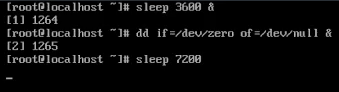
\includegraphics{1.png}
	\item Поскольку вы запустили последнюю команду без \& после неё, у вас есть 2 часа,прежде чем вы снова получите контроль над оболочкой. Введите Ctrl + z , чтобы остановить процесс: \\
	      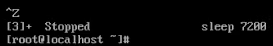
\includegraphics{2.png}
	\item Посмторите текущие задания: \\
	      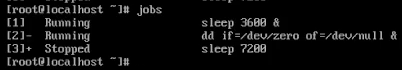
\includegraphics{3.png}
	\item Для продолжения выполнения задания 3 в фоновом режиме введите bg 3. С помощью команды jobs посмотрите изменения в статусе заданий. \\
	      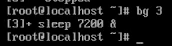
\includegraphics{4.png}
	\item Для перемещения задания 1 на передний план введите fg 1: \\
	      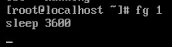
\includegraphics{5.png}
	\item Введите Ctrl + c , чтобы отменить задание 1. С помощью команды jobs посмотрите изменения в статусе заданий: \\
	      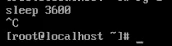
\includegraphics{6.png}
	\item Проделайте то же самое для отмены заданий 2 и 3: \\
	      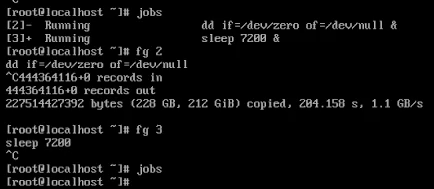
\includegraphics{7.png}
	\item Откройте второй терминал и под учётной записью своего пользователя и запустите в нём \texttt{dd if=/dev/zero of=/dev/null \&}:
	\item Введите exit, чтобы закрыть второй терминал: \\
	      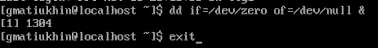
\includegraphics{8.png}
	\item На другом терминале под учётной записью своего пользователя запустите top: \\
	      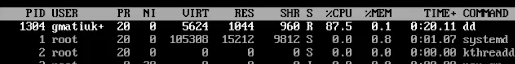
\includegraphics{9.png}
	\item Вновь запустите top и в нём используйте k , чтобы убить задание dd. После этого выйдите из top: \\
	      
\includegraphics{10.png}
\end{enumerate}

\subsection{Управление процессами}
\begin{enumerate}
	\item Получите полномочия администратора:
	\item Введите следующие команды:
	\item Посмотрите запущенные процессы: \\
	      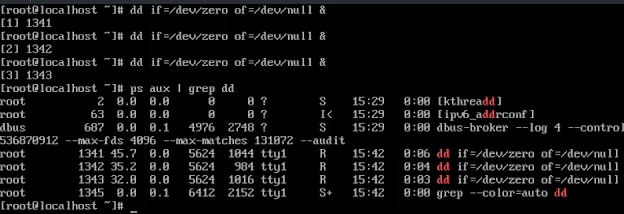
\includegraphics{11.png}
	\item Используйте PID одного из процессов dd, чтобы изменить приоритет: \\
	      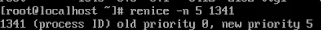
\includegraphics{12.png}
	\item Посмотрите иерархию запущенных процессов: \\
	      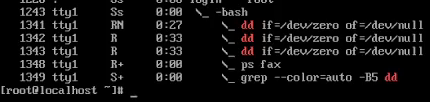
\includegraphics{13.png}
	\item Найдите PID корневой оболочки, из которой были запущены процессы dd, и завершите этот процесс: \\
	      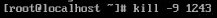
\includegraphics{14.png}
\end{enumerate}

\section{Контрольные вопросы}
\begin{enumerate}
	\item Какая команда даёт обзор всех текущих заданий оболочки? \\
	      \texttt{jobs}
	\item Как остановить текущее задание оболочки, чтобы продолжить его выполнение в фоновом режиме? \\
	      Сначала \texttt{Ctrl+z}, чтобы преостановить процесс, потом \texttt{jobs}, чтобы узнать номер процесса, потом \texttt{bg <N>}, чтобы продолжить его выполнение в фоновом режиме.
	\item Какую комбинацию клавиш можно использовать для отмены текущего задания оболочки? \\
	      \texttt{Ctrl+c}
	\item Необходимо отменить одно из начатых заданий. Доступ к оболочке, в которой в данный момент работает пользователь, невозможен. Что можно сделать, чтобы отменить задание? \\
	      Узнать \texttt{PID} процесса, используя \texttt{ps fax}, прервать процесс по \texttt{PID}, используя \texttt{kill -9 <PID>}
	\item Какая команда используется для отображения отношений между родительскими и дочерними процессами? \\
	      \texttt{ps fax}
	\item Какая команда позволит изменить приоритет процесса с идентификатором 1234 на более высокий? \\
	      \texttt{renice -5 1234}
	\item В системе в настоящее время запущено 20 процессов dd. Как проще всего остановить их все сразу? \\
	      Узнать \texttt{PID} оболочки, из которой они были запущены и остановить ее импользуя \texttt{kill -9 <shell-pid>}
	\item Какая команда позволяет остановить команду с именем mycommand? \\
	      Можно использовать \texttt{top}, чтобы найти процесс по имени. Далее, нажать \texttt{k} и ввести \texttt{PID} процесса, написанный рядом.
	\item Какая команда используется в top, чтобы убить процесс? \\
	      \texttt{k}
	\item Как запустить команду с достаточно высоким приоритетом, не рискуя, что не хватит ресурсов для других процессов?
\end{enumerate}

\section{Вывод}
В ходе выполнения данной работы я получил навыки управления системными службами операционной системы посредством \texttt{systemd}.
\end{document}
